\documentclass[10pt]{article}
\usepackage{graphicx}
\usepackage{exercise}
\usepackage{enumerate}
\usepackage{amsmath,amssymb,amsthm}
\usepackage{array}
\usepackage{listings}
\usepackage{comment}
\usepackage[toc,page]{appendix}
\newcolumntype{P}[1]{>{\centering\arraybackslash}p{#1}}

\author{Matt Piekenbrock (U00625376), \\ Jace Robinson (U00667313), \\Ning Xie (U00833572)}
\title{Did you make the Wright Choice for your College? \\
{\large CS-7830-01 - Machine Learning}}
 	
\begin{document}
\maketitle % Title page 
\clearpage % clear for TOC
\tableofcontents % TOC
\clearpage % clear for content 
\section{Introduction}
%  What problem/challenge motivates this work 
    It is well known that U.S. university students often graduate with copious amounts of financial debt. Despite the U.S. Department of Educations Mission Statement of "...promote[ing] student achievement and preparation for global competitiveness by fostering educational excellence and ensuring equal access."~\cite{Overview75:online}, college tuition rates are often far above an affordable threshold of being considered practical, which often limits many aspiring students' enrollment choices to educational institutions that seem more affordable. Even worse, students who do graduate often find themselves facing repayment obligations that far outweigh their potential income earnings. These notations collectively spark a number of questions, can we discover and explain groupings of colleges which exhibit similar characteristics? Can examining the relationship between features such as tuition costs and earnings after graduation help future students make more informed college decisions? 
    
    %These notions collectively spark a number of questions, centered around the same idea: Is college generally worth the massive financial debt that prerequisites attendance and, if so, which colleges offer truly cost-effective educations, given their tuition cost? 
    
    %     General Notions about the top 
    The average person in the U.S. may perhaps agree that students who graduate from the ``elite" colleges (i.e. Stanford, MIT, Carnegie Mellon, UC Berkeley, etc.) tend to earn more than graduates from more middle-ground universities, however, the in-depth relationships between future income and choice of university are not at all well known, nor are they intrinsically deterministic. 

% What value it brings     
    The recent manifestation of openly accessible, public-domain data sets provides an opportunity never before possible to know more about the underlying relationships regarding the true quality of college education. Using the College Scorecard data set collected by the United States Department of Education \cite{collegeScorecard}, we intend to provide a detailed `bang-for-buck" analysis into the underlying reasons regarding the relative success--or failure--graduates from particular universities of interest are facing. 
   
\section{Data Set and Packages}

The college scorecard data set \cite{collegeScorecard} is provided to the public by the U.S. Department of Education. This data set contains over a thousand features on thousands of universities since 1996. Looking closer at the data for the year 2012-13, it contains 1743 features on 7793 colleges. Some examples of colleges included are Wright State Main-Campus, Ohio State, University of Phoenix, and Harvard. The over 1700 features describe various interesting details about each college such as admission rates, ACT/SAT requirements, tuition costs, student ethnicity proportions, average student family's income levels, retention rates, debt levels, post graduation income levels, and many, many more. Some multi-class features of interest include the region (Great Lakes, New England, etc...), the locale of institution (city, suburb, town, rural), or control of institution (public, private nonprofit, private for-profit). An additional notable classification is the \textit{Carnegie Classification}, which is used to classify universities into broad groups such as large, medium, or small in population size, or for defining an undergraduate profile such as majority full-time or part-time students with low or high transfer rates. From the rich set of features this data set provides, this research project seeks to answer some exciting questions relating to the quantitative differences in colleges. 

\subsection{Data Preprocessing}

 The first step was to select a subset of the total 1743 possible features. We selected 18 features described in \ref{table:data}. These features were selected as expecting to be the most interesting for the questions explored in this report. Some of the features relate to post graduate income, debt levels, university costs, and other interesting characteristics of a university. Some of the features that were ignored in this exploration are the admission rates, ACT and SAT scores, and ethnicity proportions. The reasoning for not including these features are that our emphasis was on \textit{financial} accessibility and benefits/drawbacks of universities, and the intelligence and ethnicity proportions did not seem as relevant.

Not all features are collected for each university, while the machine learning algorithms expects data for all features to be present. Due to this, an additional subset of the data was selected, where we remove all universities which did not contain data for one or more of the desired features described in table \ref{table:data}. This brought the data from original number of universities 7793 to 1614. Some of the notable universities still in this dataset are Wright State, Ohio State, Michigan, Dayton, Harvard, and Berkeley. Some of the universities that were removed from the dataset include Stanford, Carnegie Mellon, and most specialized nursing schools (schools with nursing the name). The number of nursing schools in the original dataset is 148, while in the subset dataset there are 3 nursing schools. From inspection, many of the nursing schools did not have their tuition costs included in the dataset. Alternatives to this data preprocessing approach include data imputation, where missing data is predicted and substituted. Since there was still a large amount of data remaining after the cleaning (1614 universities), simply removing the records was sufficient.

For the experimental design, the data is partitioned into three datasets of training, validation, and testing. The training is 64\% of the data, validation is 16\%, and testing is 20\%. Both the classification and regression experiments were completed on the same partitions to allow for meaningful comparisons.

\begin{table}
\begin{center}
\begin{tabular}{ |P{4cm}|P{5cm}| }
 \hline ID & Description \\ \hline
 INSTNM & institution name \\ \hline 
 CONTROL & public, private non-profit, or private for-profit \\ \hline 
 REGION & New England,
Mid East, 
Great Lakes, 
Plains, 
Southeast,
Southwest,
Rocky Mountains, 
Far West, 
Outlying Areas
 \\ \hline 
 UGDS & enrollment of undergraduate degree seeking students\\ \hline  
 TUITIONFEE\_IN & in-state tuition \\ \hline 
 TUITIONFEE\_OUT & out-of-state tuition \\ \hline 
 TUITFTE & net tuition revenue per full-time student \\ \hline 
 AVGFACSAL & average faculty salary \\ \hline 
 C150\_4 & completion rate for first time, full-time students within 6 years \\ \hline 
 COMPL\_RPY\_5YR\_RT & One-year repayment rate for completers \\ \hline 
 PAR\_ED\_PCT\_1STGEN & percentage first-generation students \\ \hline 
 PAR\_ED\_PCT\_PS & percentage of students whose parents have post-secondary education \\ \hline 
 FAMINC & average family income \\ \hline 
 DEBT\_MDN & median debt upon start of repayment \\ \hline 
 GRAD\_DEBT\_MDN & median debt for completers \\ \hline 
 WDRAW\_DEBT\_MDN & median debt for not completed \\ \hline 
 CDR2 & two-year default rate \\ \hline 
 MN\_EARN\_WNE\_P10 & mean earnings of students working 10 years after enrollment \\ \hline 
\end{tabular}
\caption{Data Description Table}
\label{table:data}
\end{center}
\end{table}

\subsection{Software Packages and Tools}

For this project, two of the authors programmed in R (Matt and Jace) and the third programmed in Python (Ning). For R, the packages and functions primarily used were \textit{MCMCPack} for the Bayesian linear and Bayesian logistic, function \textit{glm} (built in R) for linear and logistic, \textit{ggplot} for visualizations, \textit{car} for R diagnostics. In python, library \textit{sklearn} had the support vector machine implementation.

\section{Objective}

In an effort to better understand the characteristics of college dataset, several smaller questions can be asked and answered within the scope of this project.

 \begin{enumerate}
    %\item What are the universities that provide the maximum value (to be defined) to its students?
    %\item Examine trends about Wright State, Ohio State, and University of Dayton over time. What are the post graduate income levels, and how do they relate to tuition when compared to other neighboring universities (regression/exploratory)?
    \item What are the differences between public and private schools? Look to explain these differences based on features described in table \ref{table:data}.
    \item What are the differences between schools from various regions? Look to explain these differences based on features described in table \ref{table:data}.
    \item Predict post graduate income by college based features such as family income, graduation rates, ethnicity proportions, acceptance rates, population size, debt levels, and tuition levels (regression problem). What set of features provide the best prediction accuracy?
\end{enumerate}

% What specifics, demonstrable or measurable outcomes/capabilities/techniques... provide architecture schematic; identify how you obtained innovation/novelty
The field of Machine Learning is vast; the book "Machine Learning: A Probabilistic Perspective" \cite{murphy2012machine} covers 28 major categories of the machine learning field, discretized into distinct chapters, each of which presents numerous models, methods, and statistical estimation techniques that could all potentially be used $\textit{in some way}$ to address the above goals. Although some techniques may offer advantages for specific goals compared to others (mentioned below), the correct algorithms or ``tools" to do a generalizable cost-analysis of aforementioned scorecard data are, relatively, unknown to the authors. Despite this, and following the curriculum of the class, we've chosen to include Bayesian equivalents to several of the machine learning models presented throughout the semester, including: 
\begin{enumerate}
	\item Linear Regression (Matt)
    \item Bayesian Linear Regression (Matt)
    \item Logistic Regression (Jace)
    \item Bayesian Logistic Regression (Jace)
    \item Support Vector Machine (SVM) (Ning)
\end{enumerate}

% The reasons for a Bayesian approach are manyfold; primarily, we believe inference-based techniques using probabilistic models should have a systematic framework for incorporating {\it a priori} knowledge into the calculation of the model itself, and that the probabilities estimated by such models should be built using the full degree of belief we have about the underlying data set. 

From a practical point of view, Bayesian statistics have been on the rise in popularity~\cite{ashby2006bayesian} in the past decade, and an exploration into Bayesian methods of probabilistic inference seems to be both valuable and effective to understanding more about the field of Machine Learning itself. 

A support vector machine allows for a more complex decision boundary than the logistic regression. In cases where the data is linearly separable, it is expected the two algorithms will achieve similar performance. In cases where the separation of data is more complex, a support vector machine has the advantage of being able represent non-linear boundaries in high dimension space using a \textit{kernel trick}.

% A limitation of logistic regression and SVM is the requirement of a binary output variable. In a multi-class setting, these problem can be transformed into a collection of one-versus-all binary problems. An alternative to changing the problem is to use an algorithm such as Softmax Regression which allows for a categorical decision. The performance differences of this approach versus the former will be explored. 

% In many classification settings, a binary or categorical yes or no response does not always capture the complete complexity of human reasoning. Often there are non-distinct boundaries representing a smoother transition between yes or no. Frequently people describe colleges with different levels of severity such as a \textit{great} college, \textit{good} college, \textit{okay} college, or \textit{bad} college. Through the use of \textit{Fuzzy Logic}, we are able to capture this nuanced transition from yes and no. The exploration of fuzzy logic techniques will be a \textit{time-permitting} optional investigation by the authors.

To determine the relative performance of each of the algorithms during this investigation, the following questions will be explored:

\begin{enumerate}
	\item Does the incorporation of prior knowledge in the Bayesian algorithms improve regression and classification accuracy? We use performance metrics of F1, AIC, Likelihood Ratio, F-score, $R^2$, etc. 
    \item Does an algorithm such as the SVM lead to improved classification accuracy over logistic regression? Use performance metrics of F1 and AUC.
    %\item Does the use of Softmax regression against the one-versus-all algorithms lead to improved classification accuracy? Does one-versus-all \textit{miss} meaningful information?
    %\item Can Fuzzy Logic allow for a more insightful classification of the dataset as opposed to multi-class classification using logistic regression and SVM (time-permitting)?
\end{enumerate}

% In the completion of this report, the authors and future readers are expected to have a stronger understanding of the differing characteristics of colleges around the nation. Along with the dataset analysis, readers will be exposed to how a diverse set of algorithms perform on similar problems, providing practical knowledge on the strengths and weaknesses of each of the techniques.  

The remainder of the report is separated into two major partitions, the first for classification problems, and the second for regression.
    
\section{Approach - Classification}     
    
\subsection{Classification Data Overview}

It is always recommended to perform some form exploratory analysis before applying machine learning algorithms on a dataset. The first exploration is the relationship between the 3-class public, private non-profit, and private for-profit universities. The best case scenario in these plots would be clear class separation in at least one of the features. By examining each figure, there is no feature which seems to show clear separation between the classes. For example, when looking at the first subplot, UGDS (number of undergraduate degree seeking students) versus control, there is significantly overlap in the red, green, and blue points. The only feature which shows a minor degree of separation is the TUITIONFEE\_IN (in-state tuition) versus control. It appears public schools (as shown in red) have in general lower in-state tuition than the private schools, although there are still many private schools with low tuition costs. Since no single feature separates the classes, we look towards a combination of two or more features to identify the classes.\\

\includegraphics[width=\textwidth]{figures/control-overview1}
\includegraphics[width=\textwidth]{figures/control-overview2}

In the second classification question for this dataset, we will explore the relationships between region and numerous features. Again, the best case scenario is for one or more of the classes to show separation for a single feature. As seen in the figures, the last class, outlying areas, is partially separable for features such as out-of-state tuition (TUITIONFEE\_OUT), family income (FAMINC), median graduate debt (GRAD\_DEBT\_MDN), and mean earnings 10 years after enrollment (MN\_EARN\_WNE\_P10). The means we can expect good performance for a machine learning classification of outlying areas versus the other classes. For the other eight classes, there is not any clear separation, and hence the classification problem will be much harder, requiring a combination of features to achieve separation.\\

\includegraphics[width=\textwidth]{figures/region-overview1}
\includegraphics[width=\textwidth]{figures/region-overview2}


% OPTIONAL IF WE WANT MORE DISCUSSION
% \includegraphics[width=\textwidth]{figures/ccsizset-overview1}
% \includegraphics[width=\textwidth]{figures/ccsizset-overview2}

% OPTIONAL IF WE WANT MORE DISCUSSION
% \includegraphics[width=\textwidth]{figures/ccugprof-overview1}
% \includegraphics[width=\textwidth]{figures/ccugprof-overview2}
    
\subsection{Algorithms}

For the classification tasks, there were three algorithms used, Logistic Regression, Bayesian Logistic Regression, and Support Vector Machines (SVM).

\subsubsection{Logistic Regression}

Logistic regression, one of the simplest classification algorithms often used as a first step in binary problems. It is a discriminative classifier, meaning it models the relationship of classes given some input, that is $p(y | x)$. The classes are modeled using a Bernoulli distribution, with the probability being modeled as a sigmoid function of the data and learned weights $\theta$. 

$$p(y| x, \theta) = Ber(y | sigm(\theta^T x))$$

Some of the appeals of logistic regression include easy to fit, and easy to interpret.

\subsubsection{Bayesian Logistic Regression}

Bayesian logistic regression, is a variant of logistic regression which takes advantage of the Bayesian statistics, where prior and posterior distributions are considered. In this context, we treat our parameters $\theta$ as random variables (as opposed to fixed in logistic regression), allowing for prior knowledge to be injected into the system. The goal is the estimate the posterior distribution $p(\theta | y, x)$, which can then be used to create estimates of $\hat{\theta}$. To estimate the posterior, we can apply Bayes rule to write it in terms of the prior and likelihood.

$$Y \sim p(y | x, \theta)$$
$$\theta \sim p(\theta) = \mathcal{N}(b_0, B_0^{-1})$$
$$p(\theta | y, x) \propto p(y | x, \theta)p(\theta)$$ 

where the prior is a multivariate normal with hyper-parameters mean $b_0$ and variance $B_0$. Some sophisticated techniques to set the hyperparameters include grid based searches, gradient optimization, and Bayesian optimization. In this report, \textbf{we manually select the hyperparameters based on simply intuition and subjective prior understanding of the author.} This is not a recommended approach for more serious research, but it useful to build understanding on the topic. 

As this form of Bayesian logistic regression does not have a closed-form solution for the posterior, numerical approximations must be implemented. The solution chosen is to use a Markov Chain Monte Carlo (MCMC) with Metropolis-Hastings sampling. MCMC is considered one of the top 10 most important algorithms to be created in the 20th century, due to its ability to estimate distributions, integrals, and moments. In this report, the author simply used MCMC as a black box approximation tool, without learning deep details of the algorithm. Understanding the algorithm in more detail is left as future work due to time constraints.

\subsubsection{Support Vector Machine(SVM)}

\textit{\textbf{What is SVM?}}

Support Vector Machine(SVM) is well known for solving classification problems with not very large training dataset, and could abstract nonlinear or high dimensional features from the given data. It is based on the theory of VC dimension and structural risk minimization in statistics. What it does is to “map” the original data space to a new and maybe a higher dimension, and try to find a hyperplane that could maximize the gap between different classes. Based on the way it finds the division, SVM could be considered as a kind of Maximum Margin Classifier. The reason why it’s called “Support Vector” Machine is it is the “support vectors”, which are closest to the decision boundary in the mapped space, that make the decision, since it is the support vectors that constrain the width of the margin.[1]

\textit{\textbf{Kernel}}

The kernel of SVM makes it possible to calculate the dot production in the original lower dimensional space for the higher dimensional space, which could solve the dimension explosion problem as well as reducing calculation time. Linear kernel and RBF kernel are two most commonly used ones.

\textit{\textbf{Objective Function}}

Based on the tolerance of the error, there are two different SVMs, soft-margin SVM and hard-margin SVM, and the former one is most commonly used.

The objective function for soft-margin SVM is

$$ \min_{\omega , \gamma , \xi} \left[\frac{1}{2}\left \| \omega \right \| ^2 _2 + C \sum_{i=1}^n \xi _i \right]$$
$$ s.t. (\omega ^T   x _i + \gamma)y _i \geq 1- \xi _i , \space \forall i = 1, \ldots ,n  $$
$$ \xi \geq 0, \space \forall i = 1, \ldots ,n $$

where $ \xi $ is known as the hinge loss, $ \frac{1}{2}\left \| \omega \right \| ^2 _2 $ is considered as the L2 regularization, and $ C $ is the penalty parameter for the error terms. The parameter $ C $ determines the tradeoff between increasing the margin size and ensuring the classify correctness of each training data point.

\textit{\textbf{Parameters to Tweak}}

The to-be-tweaked parameters for the SVM model I use (sklearn library, python) are 
kernel function choice
Penalty parameter $ C $
Gamma parameter for the non-linear kernel function

I choose either linear or RBF for the kernel function. For the penalty parameter $ C $, the larger $ C $ is, the more strict the classifier becomes to make the exact correct decision on each training data point. The gamma parameter determines the distribution of the data in the mapped space.
    
\section{Evaluation - Classification}

\subsection{What are the Differences between Public and Private Schools?}

The broad question explored in this section, is what are the differences between public and private schools? To answer this question, we look towards machine learning classification algorithms. \textbf{Our assumption is that if a set of features are able to accurately predict the classes correctly, then those features show some of the differences between public and private schools.} When searching for the difference between public and privates schools through exterior research (not through machine learning on this dataset), an explanation is due to differences in funding, as public schools receive funding from state taxes, while private schools do not. Most public schools have separate tuition prices for in-state tuition versus out-of-state tuition, due to the funding from the states. On the other hand, private schools have the same tuition for both in-state and out-of-state students. Based on this definition of the difference, we hypothesize that using the features of in-state tuition and out-of-state tuition in a machine learning algorithm, the two classes can be accurately separated. To check our hypothesis, we explore the problem using logistic regression, Bayesian logistic regression, and various SVM's.

\subsubsection{Tuition Only Analysis}

In the three figures below, we show the logistic regression results on the testing partition with the two input features of in-state and out-of-state tuition. If the logistic value if greater than .5, we classify as public, otherwise as private. From the first figure, we examine the logistic regression output on the data. In the top graph is the original data for in-state tuition versus the control, showing a minor degree of class separation. In the bottom graph shows the output of logistic regression (values in range 0 to 1) for each university. These figures are presented to give some insight into how the various universities are being labeled by the algorithm.

\includegraphics[width=\textwidth]{figures/test-tuition-control1}
\includegraphics[width=\textwidth]{figures/test-tuition-control2}

In this third figure, the linear decision boundary allowing for excellent separation between the classes is shown as the dashed line. The reason the private data follows a straight line is that in-state and out-of-state tuition are equal (although different values due to feature scaling). This line shows that public schools will in general have lower in-state tuition than most private schools. Additionally, public schools that have low in state tuition, will have somewhat lower out of state tuition and their private counterparts. Logistic regression is able to capture this gap between the tuitions and linearly separate the classes.

\includegraphics[width=\textwidth]{figures/test-tuition-control3}

Additionally the excellent performing confusion matrix and coefficients are shown below. Due to the collinearity among these two variables, the size of the theta values can be misleading as the regressors complement each other (one large positive and one large negative).

\begin{lstlisting}
Logistic
         Actual
Predicted   0   1
        0 214   2
        1   0 106
        		Coefficients
(Intercept)     -2.0034 
TUITIONFEE_IN  -68.1578
TUITIONFEE_OUT  47.9352
\end{lstlisting}

To compare the performance of other algorithms, we also explore Bayesian logistic regression. We experiment with three different types of prior parameters. The first parameters are uninformative, representing a lack of prior knowledge of the model. The estimated posterior distributions for each parameter is shown in the right plots below. We can note the peaks of the plots correspond to the same theta values as the logistic regression from before (-2, -70, 50). This is the desired behavior for an uninformative prior, as the likelihood dominates the estimates. The right side trace plots show the quality of the MCMC approximation. A constant variance trace (as we see in the image) means the approximation was good.

\includegraphics[width=\textwidth]{figures/tuition-uninform-densities}

Below the confusion matrix shows that Bayesian logistic regression with an uninformative prior reached the same results (with slightly different $\theta$) as the logistic regression.

\begin{lstlisting}
Bayesian Logistic Uninformative
         Actual
Predicted   0   1
        0 214   2
        1   0 106
        		Coefficients
(Intercept)     -1.998
TUITIONFEE_IN  -70.911
TUITIONFEE_OUT  50.076
\end{lstlisting}

In a second example of the Bayesian model, we attempt to select intelligent, informative priors based on our past intuitive understandings of the variables. In this case, I think schools with lower in state tuition to be more likely to be public, so there should be a negative theta value. I represent this by a negative prior mean of -.75. Following similar logic, I think schools with higher out of state tuition are more likely to be public. I again represent this with a positive prior mean of +.5. For both cases I inject a medium amount of confidence in my prior knowledge by setting the prior variance to 1. This again resulted is very similar performance results as shown in the confusion matrix. We can notice the thetas decreased significantly, while maintaining the same ratio, showing the effects of the small meaned priors bringing posterior towards zero.\\

\begin{lstlisting}
Bayesian Logistic Good
         Actual
Predicted   0   1
        0 214   3
        1   0 105
                Coefficients
(Intercept)     -1.645 
TUITIONFEE_IN  -28.394
TUITIONFEE_OUT  17.681 
\end{lstlisting}

As a third example of the Bayesian model, we purposely select an overly strong but wrong prior. We claim the opposite of our previous example, giving positive relationship between in-state-tuition of public and a negative relationship between out-of-state of public with low variances of .1 and .1 and prior means of +.5 and -.5. This incorrect prior leads to much poorer results on the data. We can see the effect of the prior on the coefficients again, as they are now quite small and the sign has flipped.

\begin{lstlisting}
Bayesian Logistic Bad
         Actual
Predicted   0   1
        0 178 100
        1  36   8
               Coefficients
(Intercept)    -0.7404 
TUITIONFEE_IN   0.5779
TUITIONFEE_OUT -4.3086 
\end{lstlisting}

% \includegraphics[width=\textwidth]{figures/tuition-inform-bad-density}
% \includegraphics[width=\textwidth]{figures/tuition-inform-good-density}

The figure below shows the linear decision boundary generated for logistic regression and three Bayesian logistic regressions. The first line in black is the logistic regression, which performs the best. The second line in green (directly on top of the black line) is Bayesian with an uninformative prior. This result is desired, showing the link between Bayesian logistic regression and logistic regression. The third line in brown is the Bayesian logistic regression with a good informative prior. Although the result is not improved, this line is able to incorporate our prior knowledge while maintaining strong performance. The last line in cyan shows Bayesian logistic with an informative but wrong prior. It is possible to include too strong of a prior with incorrect results, ultimately hindering the performance of the model.

\includegraphics[width=\textwidth]{figures/tuition-all}

Along with the logistic regression algorithms, we explore the performance of SVM. The results of the SVM's on the same problem as above with various different kernels are presented. We can note all the kernels perform well, but some have drastically different shapes.

\includegraphics[width=\textwidth]{figures/svm_1}
SVM with Linear kernel

\includegraphics[width=\textwidth]{figures/svm_2}
SVM with RBF kernel (default parameters)

\includegraphics[width=\textwidth]{figures/svm_3}
SVM with RBF kernel ($ C = 10, \gamma = 10 $)

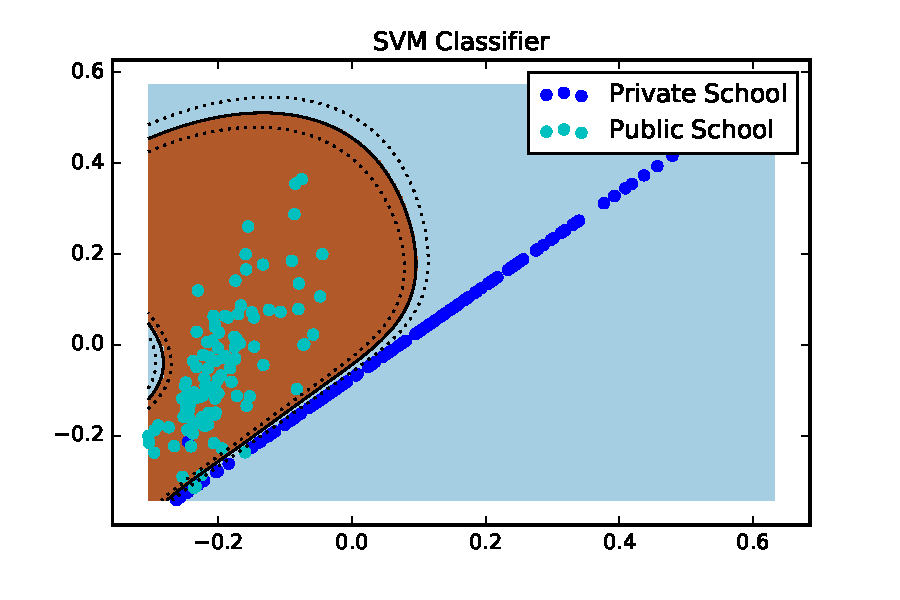
\includegraphics[width=\textwidth]{figures/svm_4}
SVM with RBF kernel ($ C = 300, \gamma = 10 $)

\includegraphics[width=\textwidth]{figures/svm_5}
SVM with RBF kernel ($ C = 300, \gamma = 600 $)

The confusion matrices provide additional insight on how the algorithm is classifying. The SVM's on various kernels had a tendency to miss-classify (false positive) the private schools more than logistic regression.

\begin{lstlisting}
Linear SVM  
         Actual
Predicted   0   1
        0 214   1
        1   7 100

RBF SVM 01  
         Actual
Predicted   0   1
        0 214   1
        1   8  99
  
RBF SVM 02 
         Actual
Predicted   0   1
        0 214   1
        1   6 101
   
RBF SVM 03 
         Actual
Predicted   0   1
        0 214   1
        1   4 103

RBF SVM 04
         Actual
Predicted   0   1
        0 215   0
        1   2 105
\end{lstlisting}

As a final summary, we show the relative performance (F1 and AIC) for all the algorithms side by side. As the classes were well separable, all algorithms performed quite well except the purposely bad prior example. As this question was \textit{easy} is a performance sense, we were unable to say one algorithm is better than the others. Returning to the original question posted in the section header, the data supports the idea that private and public schools can be described in terms of a combination of in-state-tuition and out-of-state tuition.

\begin{center}
\begin{tabular}{ |P{4cm}|P{2cm}|P{2cm}|P{2cm}| }
 \hline Features & F1 & AIC & Algorithm \\ \hline
 TUITIONFEE\_IN, TUITIONFEE\_OUT  & .99 & 14.58 & Logistic \\ \hline 
 TUITIONFEE\_IN, TUITIONFEE\_OUT & .99 & 14.58 & Bayesian Uninformative \\ \hline 
 TUITIONFEE\_IN, TUITIONFEE\_OUT & .98 & 14.58 & Bayesian Informative Good \\ \hline 
 TUITIONFEE\_IN, TUITIONFEE\_OUT & 0.441 & 167.98 & Bayesian Informative Bad \\ \hline 
 TUITIONFEE\_IN, TUITIONFEE\_OUT & 0.96 & None & Linear SVM \\ \hline 
 TUITIONFEE\_IN, TUITIONFEE\_OUT & 0.96 & 32.75 & RBF SVM 01 \\ \hline 
 TUITIONFEE\_IN, TUITIONFEE\_OUT & 0.97 & 41.55 & RBF SVM 02 \\ \hline 
 TUITIONFEE\_IN, TUITIONFEE\_OUT & 0.98 & 34.36 & RBF SVM 03 \\ \hline 
 TUITIONFEE\_IN, TUITIONFEE\_OUT & 0.99 & 79.78 & RBF SVM 04 \\ \hline 
\end{tabular}
\end{center}

\subsubsection{Excluding Tuition Analysis}

The successful separation of the public and private universities by tuition was the expected result as that is by definition one of the major distinctions between the universities. A more interesting question is can a collection of features \textit{excluding} those related to tuition separate the classes? To explore this question, we develop many models, using all possible combinations of our features. This led to 2047 unique models, with input combinations such as number of undergraduate degree seeking students, average faculty salary, and average family income. To determine the best and worst models, we use the Akaike information criterion (AIC) as covered in class, that is $-2*\text{LogLikelihood} + 2*numParams$. The features which produced the best AIC score on logistic regression were then tested on all the algorithms.

To compare the three machine learning models, we calculate the F1 score and the AICs. The first detail to notice is the best performing model is RBF SVM 02, with the highest F1 and lowest AIC. This can be due to the fact that the SVM can better model non-linear relationships between the features and the classes. The logistic regression performance slightly worse, with the Bayesian variations changing based on the quality of the prior. The last SVM RBF04 demonstrates how the model can overfit with certain poor parameters.

\begin{center}
\begin{tabular}{ |P{4cm}|P{2cm}|P{2cm}|P{2cm}| }
 \hline Features & F1 & AIC & Algorithm \\ \hline
 UGDS, AVGFACSAL, C150\_4, COMPL\_RPY\_5YR\_RT, PAR\_ED\_PCT\_1STGEN, GRAD\_DEBT\_MDN, MN\_EARN\_WNE\_P10 & 0.812 & 176.32 & Logistic \\ \hline 
 above & 0.812 & 183.913 & Bayesian Uninformative \\ \hline 
 above & 0.802 & 215.664 & Bayesian Informative Good \\ \hline 
 above & 0.441 & 282.582 & Bayesian Informative Bad \\ \hline 
 above & 0.74 & NA & Linear SVM \\ \hline 
 above & 0.62 & 194.02 & RBF SVM 01\\ \hline
 above & 0.88 & 139.55 & RBF SVM 02 \\ \hline
 above & 0.86 & 172.78 & RBF SVM 03 \\ \hline
 above & 0.29 & 233.70 & RBF SVM 04 \\ \hline
\end{tabular}
\end{center}

The provide more insight, we look at the confusion matrices for logistic, RBF SVM 02, and RBF SVM 04. In both the logistic and RBF SVM 02, the algorithm seems to classify quite well and evenly, with some false positives and some false negatives. This can be indicative of simply noisy data. On the other hand, RBF SVM 04 showed a spike in false positives, possible due to overfitting the training data.

%\begin{lstlisting}
%Logistic
%         Actual
%Predicted   0   1
%        0 192  19
 %       1  22  89 
%                   Coefficients
%(Intercept)        -1.2293
%UGDS               14.9216
%AVGFACSAL          10.6717
%C150_4             -7.4596
%COMPL_RPY_5YR_RT    9.9921
%PAR_ED_PCT_1STGEN  -2.0360 
%GRAD_DEBT_MDN      -3.8637  
%MN_EARN_WNE_P10   -14.6485
%
%Bayesian Logistic Uninformative
%         Actual
%Predicted   0   1
%        0 192  19
%        1  22  89
%                   Coefficients
%(Intercept)        -1.253
%UGDS               15.216
%AVGFACSAL          10.818
%C150_4             -7.602
%COMPL_RPY_5YR_RT   10.230
%PAR_ED_PCT_1STGEN  -2.086
%GRAD_DEBT_MDN      -3.942
%MN_EARN_WNE_P10   -14.942

%Bayesian Logistic Inform Good
%         Actual
%Predicted   0   1
%        0 201  27
%        1  13  81
%                  Coefficients
%(Intercept)       -0.8374 
%UGDS               7.0409 
%AVGFACSAL          3.8106 
%C150_4            -3.4778 
%COMPL_RPY_5YR_RT   5.0407 
%PAR_ED_PCT_1STGEN -0.6621 
%GRAD_DEBT_MDN     -3.2228 
%MN_EARN_WNE_P10   -4.0366

%Bayesian Logistic Inform Bad
%         Actual
%Predicted   0   1
%        0 209  76
%        1   5  32
%                  Coefficients
%(Intercept)       -0.6873 
%UGDS               2.6580 
%AVGFACSAL          0.5400
%C150_4            -0.9792
%COMPL_RPY_5YR_RT   2.3564
%PAR_ED_PCT_1STGEN  0.2053
%GRAD_DEBT_MDN     -1.8305
%MN_EARN_WNE_P10   -1.1835

%Linear SVM
%         Actual
%Predicted   0   1
%        0 197  18
%        1  33  74 
%        
%RBF SVM 01
%         Actual
%Predicted   0   1
%        0 207   8
%        1  55  52

%RBF SVM 02
%         Actual
%Predicted   0   1
%        0 201  14
%        1  11  96

%RBF SVM 03
%         Actual
%Predicted   0   1
%        0 198  17
%        1  13  94
%        
%RBF SVM 04
%         Actual
%Predicted   0   1
%        0 214   1
%        1  89  18
%        
%\end{lstlisting}

\begin{lstlisting}
Logistic
         Actual
Predicted   0   1
        0 192  19
        1  22  89 

RBF SVM 02
         Actual
Predicted   0   1
        0 201  14
        1  11  96
        
RBF SVM 04
         Actual
Predicted   0   1
        0 214   1
        1  89  18
\end{lstlisting}

Lastly we seek to provide meaningful interpretation of the results by examining the coefficients for logistic regression. One of the goals of this experiment was to determine if there was a grouping of features excluding tuition, which were able to separate the classes to some degree. Due to the relatively high F1 (.88) for SVM, we say there does exist a grouping of features which separate the classes. This means an answer to the original question of "What are some differences between public and private schools", can be a combination of the below features. Unfortunately, as the best grouping (and the next four below the best), all required a large number of features, making it more difficult to intuitively understand and visualize. In an attempt to intuitively understand the results, we can examine the signs of the coefficients. For example, it make sense that private schools have lower UGDS, higher graduate rates, higher debt and higher earnings. These match my prior intuition of the differences. On the other hand, I would image faculty get paid more at private schools, but the data is showing the opposite positive relationship with faculty salary.

\begin{lstlisting}
Logistic
(Intercept)        -1.2293
UGDS               14.9216
AVGFACSAL          10.6717
C150_4             -7.4596
COMPL_RPY_5YR_RT    9.9921
PAR_ED_PCT_1STGEN  -2.0360 
GRAD_DEBT_MDN      -3.8637  
MN_EARN_WNE_P10   -14.6485
\end{lstlisting}

\subsection{What are the Differences between Schools from Varying Regions?}

As a second classification analysis, we explore machine learning on the multiclass (9 classes) regions variable. The 9 classes are New England (CT, ME, MA, NH, RI, VT), Mid East (DE, DC, MD, NJ, NY, PA), Great Lakes (IL, IN, MI, OH, WI), Plains (IA, KS, MN, MO, NE, ND, SD), Southeast (AL, AR, FL, GA, KY, LA, MS, NC, SC, TN, VA, WV), Southwest (AZ, NM, OK, TX), Rocky Mountains (CO, ID, MT, UT, WY), Far West (AK, CA, HI, NV, OR, WA), and Outlying Areas (AS, FM, GU, MH, MP, PR, PW, VI). Similar to the public versus private analysis, we explore all possible combinations of features of the logistic regression, and use AIC to determine which set of features produce the best results. The implementation of logistic regression in this report only allowed for binary classes, so the problem was converted to multiclass as one versus all nine times. An alternative not included in this report is multinomial logistic regression, which is better built for multiple classes than the binary, one-versus-all implementation of logistic regression. Unfortunately, for eight of the experiments (the first eight classes), there was not a combination of features which produced strong results. Due to the one-versus-all approach, there was severe class imbalance for each experiment.

An example of one of the poor performing logistic regression examples is shown below (New England versus other). As we can see, the F1 is 0 and all of the data is classified as class 0 (other) in the confusion matrix. This can be attributed to bad class imbalance and lack of linearly separable features.

\begin{center}
\begin{tabular}{ |P{4cm}|P{2cm}|P{2cm}|P{2cm}| }
 \hline Features & F1 & AIC & Algorithm \\ \hline
 C150\_4, FAMINC  & 0 & 105.325 & Logistic \\ \hline 
\end{tabular}
\end{center}

\begin{lstlisting}
         Actual
Predicted   0   1
        0 310  13
\end{lstlisting}

For one of the classes, the Outlying Areas (class 9) versus other, logistic regression was able to very accurately classify the data despite severe class imbalance. The best performing logistic regression model by AIC is shown below. The high F1 (.857) despite the severe class imbalance (see confusion matrix) demonstrates the strong results. The largely negative coefficents show how the outlying regions have low out-of-state tuition, low average faculty salary, and low debt for students who did not graduate.

\begin{center}
\begin{tabular}{ |P{4cm}|P{2cm}|P{2cm}|P{2cm}| }
 \hline Features & F1 & AIC & Algorithm \\ \hline
 TUITIONFEE\_OUT, AVGFACSAL, WDRAW\_DEBT\_MDN  & 0.857 & 14.874 & Logistic \\ \hline 
\end{tabular}
\end{center}

\begin{lstlisting}
         Actual
Predicted   0   1
        0 315   0
        1   2   6
                Coefficients
(Intercept)     -19.246 
TUITIONFEE_OUT  -39.041
AVGFACSAL       -12.206
WDRAW_DEBT_MDN  -36.153 
\end{lstlisting}

As an additional investigation, we look at the results of the fourth best model by AIC with two input features. In the figure, the linear decision boundary is presented. The is a clear separation in the classes, as the outlying universities have a combined low out-of-state tuition and low average faculty salary.

%\includegraphics[width=\textwidth]{figures/outlying1}
%\includegraphics[width=\textwidth]{figures/outlying2}
\includegraphics[width=\textwidth]{figures/outlying3}

As an alternative to the one-versus-all approach, we perform multiclass classification using SVM. This experiment used all of the features to perform the classification The nine by nine confusion matrix and F1 scores are shown below. To examine the performance, we focus on the size of the diagonal elements relative to the rest of the classes. We can notice the larger numbers (3,25,25,10,51,etc...), showing the positive results. This is much better than the one versus all, as at least some of the data is being classified correctly. We can see an average F1 score of about .4 among all the classes.

\begin{lstlisting}
SVM(Best performance)
         	Actual
Predicted   		1  2  3  4  5  6  7  8  9
		1	3  5  2  0  2  0  0  1  0
		2	7 25  6  1  6  2  0  4  0
		3	4  8 25  2 15  1  1  1  0
		4	1  4  6 10  4  1  0  0  0
		5	3  6 17  6 51  6  1  2  0
		6	1  3  3  1 18  6  0  3  0
		7	0  0  1  1  3  0  1  1  0
		8	0  7  5  4 10  2  1  7  0
		9	0  0  0  0  0  0  0  0  6

F1 for Each Class
	0.18749999999999997
        0.45871559633027525
        0.4098360655737705
        0.39215686274509803
        0.5074626865671642
        0.22641509433962265
        0.18181818181818182
        0.25454545454545452
        1.0

\end{lstlisting}

In conclusion, there appears to be a small degree separation in the nine regions, but since the data is highly noisy, the F1 scores are still low. There was not as much separation in the regions as one might think. For example, we expected the far west region to have clear separation in some features such as earnings due to the higher cost of living, but this was not the case. Lastly the multiclass SVM performed significantly better than the one-versus-all approach.

% ------------------------------------------------------------------------------------
% START REGRESSION -- MATTS SECTION -------------------
% ------------------------------------------------------------------------------------
\section{Approach - Linear Regression}

\subsection{Regression Overview}
In a simple linear regression (SLR) model, the target random variable $Y$ given the regressor random variable(s) $X$ might be implemented as follows: 

$$ Y = \beta_0 + \beta_1 x + \epsilon $$

where $\beta_0 + \beta_1$ are the parameters of model, corresponding to the intercept and slope, respectively, and where $\epsilon$ is a random variable that is *assumed* to be distributed with $E(\epsilon) = 0$ and $Var(\epsilon) = \sigma^2$\cite{murphy2012machine}. In the SLR model, the error distance is described by $\epsilon$, which I may also call {\it residuals}, are assumed to be independent and identically normally distributed around the regression line with some variance parameter $\sigma^2$, a.k.a

$$ \epsilon_i \thicksim N(0, \sigma^2) $$

It's well known that linear regression is often generalized to allow for multiple variables, additional complexity, etc., allowing the simple expression above to be rewritten using vector notation: 

$$ y_i = x_{i}^T \beta + \epsilon_i $$

Under this model, the error term $\epsilon$ is assumed to be described sufficiently by the variance of the model $\sigma^2$, which is known as the {\it homogeneous variance assumption} (also called the assumption homoscedasticity). Yet despite the often understated assumption, many data that exists fails to meet this criterion. It is natural to think that changes in the value of the predictors used in the model may also result in changes in the variance of the response variable(s) at those values. 

Specifically, in the college scorecard data set, I am interested in modeling the average earnings of students per university 10 years after enrolling as a function of the tuition cost of the school. These variables are described by the MN\_EARN\_WNE\_P10 and TUITIONFEE\_IN, respectively. Below is an example of the what these variables look like in the data, and where relatively well-known and neighboring universities stand compared to WSU: 

\includegraphics[width=\textwidth]{figures/schools2}

Discussion regarding the school locations will occur during the presentation of the following results. For the rest of this section, I will introduce the mathematical notation regarding Bayesian Linear Regression using conjugate priors, tying each term into its english interpretation (when possible) with the college scorecard data set, starting with just mean earnings as a function of tuition cost. 

\subsection{Bayesian Linear Regression}
In simple linear regression (SLR), $x_{i}^T$ represents the tuition cost, $\beta$ the slope+intercept parameters of the model, and $\epsilon_i$ represents the residual between the model and the data, whose variation is described by:
$$\epsilon_i \thicksim N(0, \sigma^2) $$

Where $\sigma^2$ can be estimated by simply looking at the variance of the residuals. Because the structure of the data is assumed to be normal with fixed variance $sigma^2$, I plotted the first 3 standard deviations of the SLR model on the data. 

\includegraphics[width=\textwidth]{figures/SLR}

There are a number of assumptions made when building the linear regression model (linearity between mean response variables and regressors, constant variance, insignificant amount of multicollinearity, etc., assumptions of normality in residual, etc.). My goal is to use Bayesian linear regression to  address at least a few of these. 

\subsubsection{Linearity}
Looking at just the p-value (for now) for the basic linear regression model of tuition vs. mean earnings, I get some summary results that look like this: 

\begin{center}
\begin{lstlisting}
Residuals:
     Min       1Q   Median       3Q      Max 
-0.20121 -0.05919 -0.01298  0.05599  0.69880 

Coefficients:
                Estimate Std. Error t value Pr(>|t|)    
(Intercept)   -0.0002527  0.0028892  -0.087     0.93    
TUITIONFEE_IN  0.1731969  0.0132247  13.097   <2e-16 ***
---
Signif. codes: 0 * 0.001 * 0.01 * 0.05 * 0.1 * 1

Residual standard error: 0.09286 on 1031 degrees of freedom
Multiple R-squared:  0.1426,	Adjusted R-squared:  0.1418 
F-statistic: 171.5 on 1 and 1031 DF,  p-value: < 2.2e-16
\end{lstlisting}
\end{center}

In terms of assessing the linearity assumption, tuition was found to indeed be a very significant factor in the earnings of the a student 10 years after enrolling. For now, I conclude that the assumption of some kind of linear relationship between tuition and earnings is valid, and move on to the next assumption. 

\subsubsection{Normality of Residuals}
The residual errors of the linear regression model are assumed to be distributed as $\mathcal{N}(0, \sigma^2)$ where $\sigma^2$ is some fixed variance. To assess whether the errors seem to be normally distributed, I use a QQ plot. 

\includegraphics[width=\textwidth]{figures/qq_plot}

Ideally, the (studentized) residuals should fall as close to the center (solid) line as possible. They appear to not deviate so far as to conclude that assumptions of normality are invalid, however the F-score, a related measure for testing the equality of variances between the regressors and the response, is very high (1 would indicate equality in variance). On top of that, the $R-squared$ value, which \cite{walpole1993probability} cites as "the proportion of the variation explained by the model", is particularly poor, indicating that although there may be a significant effect of tuition on the mean earnings of a individual 10 years after enrolling, that effect seems particularly small. Nonetheless, judging the assumption of normality of residuals strictly qualitatively, I conclude that assuming normality is a decent assumption to make. 

\subsubsection{Homoscedasticity}
I posit that the low $R^2$ value is primarily being affected by both outliers towards the upper-end of the tuition quantiles and the lower end as well. Specialized schools like low-cost Nursing and Pharmacy schools are producing high-earning students at impressively low tuition rates, and the (better) Ivy League schools are produced students that make almost exponentially more money on average than the average college graduate. Because of this, it would appear that the assumption of constant variance between observations is most likely wrong. To test this, I used the Breusch-Pagan hypothesis test for Homoscedasticity (null hypothesis), as recommended by Cook \cite{cook1983diagnostics}. 
\begin{lstlisting}
	Non-constant Variance Score Test 
	Variance formula: ~ fitted.values 
	Chisquare = 64.00601    Df = 1     p = 1.2404e-15 
\end{lstlisting}

Immediate results show that tests for homoscedasticity fail dramatically; it seems it is perhaps an incorrect assumption to assume that the variation of earnings as the tuition changes is constant. However, as noted in \cite{breusch1979simple}, this test only indicates whether the variance in the residual is constant; it {\it is possible that there is a linear relationship between the variances of the residual and the independent variable(s)}. 

\subsection{Estimating the Posteriors (unknown variance)}
Bayesian statistics relies on the notion of a {\it prior} and a {\it likelihood} function in combination to produce a (hopefully) more accurate "predictive posterior density", which I interpret simply as a probability distribution that factors in {\bf reasonable} bias in the form of prior distribution as a means of more accurately describing the underlying structure in which the data was formed. The general form, as is well known, of the Bayesian formulation is as follows: 

$$ P(A \mid B) = \frac{P(B \mid A) \times P(A)}{ P(B) } $$

Where $P(A \mid B)$ represents the posterior, $P(B \mid A)$ represents the likelihood, $P(A)$ represents the prior, and $P(B)$ represent the marginal distribution of $B$. 

In the case of linear regression, I would like to use prior information to influence the parameterization of the SLR model such that the model may reflect my assumptions about the data more accurately. That is, I want the $\sigma$ term in the formulation of the residual $\epsilon_i$: 

$$ \epsilon_i \thicksim N(0, \sigma^2) $$
 
Formulating this in the Bayesian way requires a likelihood function for the SLR model and a set of prior distributions that are conjugate the likelihood (for an analytic solution). Following \cite{murphy2012machine}, the posterior distribution of interest is defined as 
$$ P(\beta, \sigma^2 \mid y, X) $$
which, through Bayes Rule, is proportional to:  
$$P(y \mid X, \beta, \sigma^2) P(\beta \mid \sigma^2) P(\sigma^2)$$

The likelihood of the regression model is given by: 
$$ P(y \mid X, \beta, \sigma^2) \propto (\sigma^2)^{n/2} exp(-\frac{1}{2\sigma^2}(y - X \beta)^T (y - X \beta))$$
which indicates the probability of the model given the data and the parameterization of the model. Of particular interest  are the prior distributions that allow me to make a model more flexible with respect to assuming the $\beta$ parameters can be influenced by prior domain-specific knowledge.

% The prior on the effects parameters requires knowledge of the variance of residuals if informative priors are to be used. Thus=, I describe the prior on $sigma$ as follows:  If I assume the variance of the population of schools is unknown, I can arrive at an analytic solution using an uninformative prior through the use of the inverse gamma distribution, defined as: 
% $$f(x; \alpha, \beta) = \frac{\beta^{\alpha}}{\Gamma{(\alpha)}}x^{-\alpha - 1} exp(-\frac{\beta}{x})$$
% Where $\Gamma$ corresponds to the gamma function $\Gamma{(n)} = (n-1)!$.
Assuming the use of a conjugate prior, Murphy \cite{murphy2012machine} shows that when $\sigma^2$ is unknown, 
% $$f(x; \alpha, \beta) = \frac{\beta^{\alpha}}{\Gamma{(\alpha)}}x^{-\alpha - 1} exp(-\frac{\beta}{x})
$$ P(\beta \mid \sigma^2) \propto (\sigma^2)^{-\frac{k}{2}} exp(-\frac{1}{2 \sigma^2}(\beta - \mu_0)^T \Lambda_0 (\beta - \mu_0))$$
$$ \propto \mathcal{N}(\beta_n, \sigma^2 \Lambda_n^{-1})$$
and, similarly, 
$$ P(\sigma) \propto f(x; \alpha, \beta) = \frac{\beta^{\alpha}}{\Gamma{(\alpha)}}x^{-\alpha - 1} exp(-\frac{\beta}{x})$$
$$ \propto \text{Inv-Gamma}(a_0, b_0)$$
This simplifies the calculation significantly, as now the Bayesian formulation of Linear Regression can be encapsulated as just: 
$$ \text{Posterior} \propto \mathcal{N}(\beta_n, \sigma^2 \Lambda_n^{-1}) \times \text{Inv-Gamma}(a_0, b_0) $$
Noting the variables that are not used in the SLR model, the entire course of BLR can thus be described by 4 update questions: 
$$ \Lambda_n = (X^{T} X + \Lambda_0) $$
$$ \beta_n =  (X^T X + \Lambda_0)^{-1} (\Lambda_0 \beta_0 + X^T y) $$
$$ a_n = a_0 + \frac{n}{2} $$
$$ b_n = b_0 + \frac{1}{2}(y^T y + \beta_0^T \Lambda_0 \beta_0 - \beta_n^T \Lambda_n \beta_n ) $$
where $\Lambda_0$ is interpreted as the prior precision matrix, the inverse of the prior (assumed) variance on the parameters, and $\beta_0$ corresponds to the prior distribution on the intercept and effects parameters. The hyper-parameters $a_0$ and $b_0$ are well known to be difficult to have linguistic translations, but setting both to 0 corresponds to uninformative prior on $\sigma^2$. 

\subsection{Estimating the Posteriors (known variance)}
The above set of derived equations are used to do Bayesian inference in the context where the variance of the observations were assumed to be unknown. This was shown through the use of an uninformative prior, where the precision matrix $\Lambda_0$ was set to $\frac{1}{N} X^{T} X$, corresponding to the unit information prior\cite{kass1995reference}. These results were then shown to correspond almost identically to the ``frequentist'' or classical method of linear regression, with minor differences in the computed confidence and credible intervals--but this isn't entirely useful. The assumptions made by the Bayesian model with the uninformative prior are the same as the classical linear regression model; the only benefit to BLR seems to be the slightly more conservative credible intervals and the ability get a quantile estimate of the variance of the residuals. 

Perhaps a more interesting model would be one that uses {\it informative} prior. As shown in section 7.6.1 in ``Machine Learning: A Probablistic Perspective'' \cite{murphy2012machine}, this equates to adjusting (primarily) the update equations on the prior variance of the residuals and the initial guess on the $\beta$ parameters {\it using information about the variance of the training data set to guess on the variance of the residuals}. Using this methodology, the testing data set can be used ``online'' to dynamically give error bounds on the distributions centered at the regression line. Specifically, by adjusting $\beta$ and $\Lambda_n$ with the following equations:
$$ \beta = \Lambda_n^{-1} \Lambda_0 \beta_0 + \frac{1}{\sigma^2} \Lambda_n^{-1} X^{T} y $$
$$ \Lambda_n^{-1} = \sigma^2 (\sigma^2 \Lambda_0 + X^{T} X)^{-1}$$

Recalling that $\Lambda_n^{-1}$ is simply the prior variance of the residuals and $\Lambda_0$ is the precision matrix of the prior (strength of the prior), these equations allow prior assumptions of regressors impact on the response variables to be factored in a Bayesian way. {\it This allows me to address the incorrect assumptions of constant variance} through the hyper-parameters $\Lambda_0$ and the initial guesses of the effects of the regressors on mean earnings, $\beta_0$. 

Starting with $\beta_0$, I think that it's reasonable to assume that tuition, for example, has a positive correlation with mean earnings, such that for every 10\% increase in the tuition, there's on average a 5\% increase in mean earnings after 10 years. I think this is reasonable because there seems to be an impression that better schools cost more money, and many people seem to prefer better schools not just because of the curricula but because of the social connections that the individuals are such schools may have with more influential figures in industry, academia, etc. I also think that, minimally, nearly everyone should be able to make about \$30,000 10 years out of college, regardless of the degree (intercept prediction).

I believe my assumptions to be fairly accurate, so I decided to increase the impact the prior has on the posterior [marginals] by scaling $\Lambda_0$ appropriately. The {\it uninformative} way of creating a precision matrix would be to take the inverse of the unit information prior used previously, which is just the scaled-sum-of-squares matrix $\frac{1}{N} X^{T}X$. Instead, I elected to set the prior parameter $\Lambda_0$ as the inverse of the identity matrix scaled to my the subjective confidence I have in my prior assumptions, $\tau$: 

$$ \Lambda_0 = (\tau^2 I)^{-1} $$

Murphy notes that $\tau$ in this case acts in a similar way as $\lambda$ is used in regularization as a means of preventing overfitting, where, in certain conditions, the Bayesian estimation of the posterior mean actually reduces to regularized ``ridge regression'' with $\lambda = \frac{\sigma^2}{\tau^2}$. I thus interpreted $tau$ to be a scaling parameter that allows the variance of the normals along the regression line to be smoothed out to either over-or-underfit, based on the setting of $\tau$. I think that reported earning collected via the tax system can be a bit misleading, Murphy doesn't recommend any particular techniques, so I chose to scale my precision matrix based on the (scaled) difference in variance between the testing and training data sets regarding tuition, just because that seemed to make intuitive sense to me. 

\section{Evaluation - Linear Regression}
\subsection{Posterior Predictive (unknown variance)}

To begin doing Bayesian estimation, prior parameters need to be set. I parametrized my prior parameters as $a_n = 0$, $b_n = 0$, and $\Lambda_0 = \frac{1}{n} X^T X$, corresponding to the unit information prior \cite{kass1995reference} and the recommendations of Murphy \cite{murphy2012machine} for uninformative cases. Then, following the formulation of the posterior shown in the {\bf Approach - Linear Regression} section, I computed the posterior analytically, and compared the results with results computed via MCMC in R, of which the MCMC results are shown below:

\includegraphics[width=\textwidth]{figures/mcmc2}

The posterior marginals shed some light on the ``true'' distributions of each variable. From the marginals, it appears that I can be fairly confident that the average earnings for even the lowest-ranked universities (intercept) would be around \$36,500, with there being about a 0.50 increase in earnings for every dollar spent on tuition. All three of the MCMC chains generated 10,000 samples after a 1,000 sample burnin period. The trace plots (left) qualitatively show that the marginal posteriors have likely not diverged, as exhibited by the relatively constant variance of the generated samples. To see the difference in the parameters estimated from both models, I plotted both the SLR (blue) and BLR(red) models against the training data set, with the $1^{st}$ standard deviation plotted in dashed lines for both. Note the small but noticeable difference in the size of the BLR model's standard deviation (easier to see at the very left side of the figure).  

The marginal posteriors themselves capture more information regarding how the parameter of the model are distributed, however to arrive at a useful regression model, static parameters need to be picked. For this task, I used (approximate) the {\it maximum a posteriori} estimates of the parameters $\beta$ and $\sigma^2$. The model itself is shown on the figure below for tuition and earnings: 

\includegraphics[width=\textwidth]{figures/blr_slr}

\begin{lstlisting}
                     2.5 %       97.5 %
(Intercept)   3.505882e+04 3.761742e+04
TUITIONFEE_IN 4.339889e-01 5.665174e-01
                      2.5%        97.5%
(Intercept)   3.506053e+04 3.761770e+04
TUITIONFEE_IN 4.344142e-01 5.672595e-01
sigma2        1.104268e+08 1.312099e+08
\end{lstlisting}

95\% confidence (top) and credible intervals (bottom) of both models are listed above as well. Note that with the BLR model, unlike SLR, the reported quantile estimates are referred to as {\it credible} intervals, as opposed to confidence intervals, and (unlike the SLR model) can be computed for $\sigma^2$ estimates as well as for the $\beta$ parameters. You can see that the intervals are very close to each other in every case, with the Bayesian credible intervals being slightly larger than the normal confidence intervals. The fact that these are very close, despite very different formulations, is known to be normal behavior when using an uninformative prior\cite{murphy2012machine}. It's also worthy to note that Bayesian credible intervals are generally considered more conservative\cite{curran2005introduction}.  

\subsection{Posterior Predictive (known variance)}
The results (the first standard deviation of the estimated posterior residual distributions $\mathcal{N}(0, \sigma_N^2)$, are shown per every 15 data points) are shown below: 
\includegraphics[width=\textwidth]{figures/blr}
The figure above depicts the result of the (regularized) Bayesian Linear regression, with the testing data set plotted as black points. As shown above, the adaptive variance in the parameterization of the residuals distribution appears to capture the spread of the data on more local levels--one standard deviation in BLR captures more of the points variations than the basic model with constant variance. This directly goes back to the original hypothesis that resulted from the Breusch-Pagan hypothesis test for conditional heteroskedasticity (alternative hypothesis); adapting the residual variance to be a function of the independent variable(s) may yield a better model. 

The posterior predictive density for the residual variance term $\sigma^2$ was computed using: 
	$$\sigma^2(\hat{X}) = \sigma^2 + \hat{X}^{T} V_n \hat{X} $$ 
where $\sigma^2$ represents the variance from the training data, $\hat{X}$ represents the training data, and $V_n$ is the above mentioned covariance matrix on the hyper-parameters. It's important to note that, as mentioned by \cite{murphy2012machine}, the error bars shown above were calculated using both training data set and the testing set actively factored in when the posterior predictive is computed, and essentially represents the {\it uncertainty of the testing set as a function of the training set}. To quote Kevin Murphy in section 7.6.2: ``This is important for applications such as active learning, where we want to model what we don't know as well as what we do.''

Although the well-known $R^2$ measure may be interpreted as the amount of the datas variation explained by the model\cite{walpole1993probability}, because the means are always centered at the regression line, the coefficient of determination ($R^2$), the total corrected sum of squares ($SST$), the error sum of squares ($SSE$), and the root-mean-square error ($RMSE$) seem to all be measures of fit based on the assumption of constant variance, as per-observation variance term are not included in any of the calculations. 

Instead of using distance-based measures, using the $\sigma^2$ estimates at every point, I computed the sum of the likelihood values for both the constant variance case vs. the bayesian-estimated variance values, which ended up being 485.4279 and 507.546, respectively. The results do suggest that the Bayesian Regression case captured more of the variance of the observations in the test set than the SLR model, indicating that Bayesian linear regression can indeed prove superior in many cases. By taking the difference between the computed likelihoods of the given data and normalizing by the number of testing samples, an average likelihood gained (probability of observation given the model) increased by a factor of 0.06868975. Thus, with an unoptimized, informative prior, I was able to explain observations outside of the training set by an additional 6\%. 

Analyzing the SLR model, to go back to the original problem extension of predicting mean earnings based on features like faculty salary, tuition cost, family income, etc., we took what we believed to be the most relevant features in the dataset and ran a multiple-regression model using these variables, with the results shown below:  

\begin{lstlisting}
Coefficients:
                Estimate Std. Error t value Pr(>|t|)    
(Intercept)    2.477e+04  1.059e+03  23.393  < 2e-16 ***
FAMINC         1.317e-01  2.080e-02   6.332 3.61e-10 ***
C150_4        -4.363e+03  2.385e+03  -1.829   0.0677 .  
TUITIONFEE_IN  2.844e-01  3.650e-02   7.793 1.60e-14 ***
AVGFACSAL      2.005e+00  1.858e-01  10.794  < 2e-16 ***
DEBT_MDN      -2.089e-01  9.361e-02  -2.232   0.0258 *  
---
Signif. codes:  0 * 0.001 * 0.01 * 0.05 * 0.1 * 1

Residual standard error: 9304 on 1027 degrees of freedom
Multiple R-squared:  0.4087,	Adjusted R-squared:  0.4058 
F-statistic: 141.9 on 5 and 1027 DF,  p-value: < 2.2e-16
\end{lstlisting}
For posteriority sake, the confidence and credibility intervals were computed using average family income, graduation rate\footnote{Calculated as the percentage of students that graduate within 150\% of the number of hours required by their degree.}, tuition cost, average faculty salary, and median debt were used as regressors to predict the mean earnings of students working 10 years after enrollment. The results show similar margins. 
\begin{lstlisting}
                      2.5 %        97.5 %
(Intercept)    2.269298e+04  2.684873e+04
FAMINC         9.089244e-02  1.725221e-01
C150_4        -9.043560e+03  3.184399e+02
TUITIONFEE_IN  2.128264e-01  3.560765e-01
AVGFACSAL      1.640752e+00  2.369880e+00
DEBT_MDN      -3.926032e-01 -2.523721e-02
                       2.5%         97.5%
(Intercept)    2.271052e+04  2.683462e+04
FAMINC         9.096594e-02  1.721618e-01
C150_4        -9.104433e+03  2.964682e+02
TUITIONFEE_IN  2.112052e-01  3.568618e-01
AVGFACSAL      1.637181e+00  2.364305e+00
DEBT_MDN      -3.954695e-01 -2.381564e-02
sigma2         7.957143e+07  9.459787e+07
\end{lstlisting}
Of these features, as shown above, family income, tuition cost, and faculty salary were the only features to have very significant p-values, indicating that variables like median debt and graduation {\bf rates} have less of an impact of the future earnings of graduates than, for example, the faculty salary. Inspection of the Variance Inflation Factors, shown below, indicate that there doesn't seem to be significant amounts of multicollinearity in the model, leading me to believe the adjusted $R^2$ value as genuine. 
\begin{center}
 \begin{tabular}{|c c c c c|} 
 \hline
 Family Income & Grad. Rate & Tuition cost & Faculty Salary & Median Debt \\  [0.5ex] 
 \hline
 285490 & 2.520840 & 1.622669 & 2.180178 & 2.264671  \\ 
 \hline 
\end{tabular}
\end{center}
From these results I gather the following theories: every university will have students that drop out, as there doesn't seem to be a very significant relationship between the schools graduation rate and the mean earnings of the student 10 years after enrolling. Median debt doesn't seem to have a significant impact either--perhaps everyone is in debt, regardless of the future potential earnings. Conversely, coming from a wealthier family certainly seems to have an impact on future earnings, as does tuition cost. An important question remains, however--just because a student may be statistically more likely to make more money 10 years after enrolling in a very higher tuition university, is the amount of tuition he\/she pays worth the (relatively) small increase in {\it possible} earning potential?  

\begin{comment}

\begin{appendices}
  \section{Milestones}
  
  \begin{center}
\begin{tabular}{| P{5.5cm} | P{2cm} | P{1.5cm} | P{2cm} |}
 \hline Task & Projected Completion Date & Assigned Member & Completion \\ 
 \hline Implement Bayesian Linear Regression on sample dataset & 10-27-16 & Matt & \\  
 \hline Implement Bayesian Logistic Regression on sample dataset & 10-27-16 & Jace & \\
 \hline Implement SVM on sample dataset & 10-27-16 & Ning & \\
 \hline Analyze College Scorecard dataset with Linear Regression & 11-3-16 & Matt & \\
 \hline Analyze College Scorecard dataset with Logistic Regression & 11-3-16 & Jace & \\
  \hline Implement SoftMax on sample dataset & 11-3-16 & Ning & \\
 \hline Analyze College Scorecard dataset with Bayesian Linear Regression & 11-10-16 & Matt & \\
 \hline Analyze College Scorecard dataset with Bayesian Logistic Regression & 11-10-16 & Jace & \\
  \hline Analyze College Scorecard dataset with SVM and Softmax & 11-10-16 & Ning & \\
 \hline Create nearly completed regression analysis report & 11-17-16 & Matt & \\
 \hline Create nearly completed logistic regression analysis report & 11-17-16 & Jace & \\
 \hline Create nearly completed SVM and Softmax analysis report & 11-17-16 & Ning & \\
 \hline Merge analysis into single report & 11-24-16 & ALL & \\
 \hline
\end{tabular}
\end{center}
  
\end{appendices}

\end{comment}
\clearpage
\bibliographystyle{abbrv}
\bibliography{report}

\end{document}
